\documentclass{article}

\usepackage[a4paper,margin=3cm]{geometry}
\usepackage{amsmath}
\usepackage{mathtools}
\usepackage{tikz}
\usepackage{pgf-pie}
\usepackage{tikz-cd}
\usepackage{cancel}
\usepackage{setspace}
\usepackage[fontsize=16pt]{fontsize}
\usepackage{indentfirst}

\author{Mike McLennan}
\date{}
\title{simple\\Multiplication\\
\vspace{28pt}
\begin{normalsize}Applied Scholastics, Ferndale WA \end{normalsize}}

\begin{document}

\maketitle
\pagebreak
\tableofcontents
\pagebreak
\begin{spacing}{1.25}

\section{Multiplication}
Multiply means to add a number to itself many times. It is from Latin. Multi- means many, and -ply means fold, so multiply means folded many times.\\

Multiplication is called times, because it is adding a number to itself many times.\\

The times symbol is $\times$: 
$\overbrace{8+8+8+8}^{\textrm{8 added to itself 4 times}}= 8 \times 4 = 32$\\

Sometimes a dot ( . ) or a raised dot ($\text{ }\cdot$\text{ })is used for times because it can be confused for the letter x, and because it is shorter.
Sometimes the times symbol is just left out so if two things are next to each other in a maths statement it is assumed that times is meant.\\

The result of multiplying is called the product. The product of 2 and 4 is 8, for example.

\newpage

\section{Skip Counting}
Learning skip counting is the first step in learning to multiply. These are called the multiples of a number.\\

Practice until you can skip count all the way to 100 for any number without looking.\\

Practice counting by twos all the way to 100:\\
2, 4, 6, 8, 10, 12, 14, 16, 18, 20, 22, 24, 26, 28, 30, 32, 34, 36, 38, 40, 42, 44, 46, 48, 50, 52, 54, 56, 58, 60, 62, 64, 66, 68, 70, 72, 74, 76, 78, 80, 82, 84, 86, 88, 90, 92, 94, 96, 98, 100.\\

You can see this on a number line.

\begin{center}
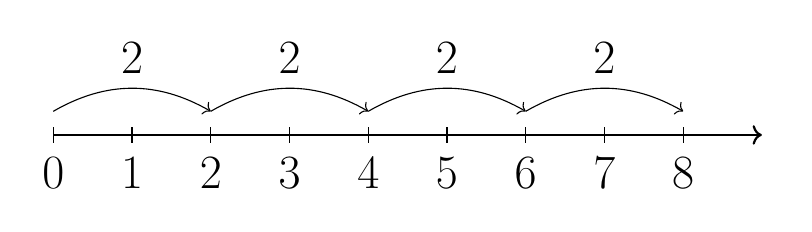
\begin{tikzpicture}
\draw[thick, ->] (0,0) -- (9,0) node[below] {$\ $};
\foreach \n in {0,1,2,3,4,5,6,7,8} {\draw (\n,0.1) -- (\n,-0.1) node[below] {$\n$};}
\draw[->, bend left=30] (0,0.3) to node[above] {$2$} (2,0.3);
\draw[->, bend left=30] (2,0.3) to node[above] {$2$} (4,0.3);
\draw[->, bend left=30] (4,0.3) to node[above] {$2$} (6,0.3);
\draw[->, bend left=30] (6,0.3) to node[above] {$2$} (8,0.3);
\end{tikzpicture}
\end{center}

Practice counting by threes all the way to 100:\\
3, 6, 9, 12, 15, 18, 21, 24, 27, 30, 33, 36, 39, 42, 45, 48, 51, 54, 57, 60, 63, 66, 69, 72, 75, 78, 81, 84, 87, 90, 93, 96, 99.

\begin{center}
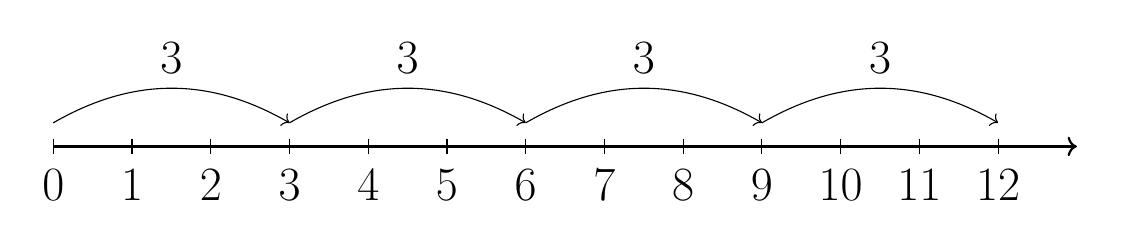
\begin{tikzpicture}
\draw[thick, ->] (0,0) -- (13,0) node[below] {$\ $};
\foreach \n in {0,1,2,3,4,5,6,7,8,9,10,11,12} {\draw (\n,0.1) -- (\n,-0.1) node[below] {$\n$};}
\draw[->, bend left=30] (0,0.3) to node[above] {$3$} (3,0.3);
\draw[->, bend left=30] (3,0.3) to node[above] {$3$} (6,0.3);
\draw[->, bend left=30] (6,0.3) to node[above] {$3$} (9,0.3);
\draw[->, bend left=30] (9,0.3) to node[above] {$3$} (12,0.3);
\end{tikzpicture}
\end{center}

\newpage

Practice counting by fours all the way to 100:\\
4, 8, 12, 16, 20, 24, 28, 32, 36, 40, 44, 48, 52, 56, 60, 64, 68, 72, 76, 80, 84, 88, 92, 96, 100.

\begin{center}
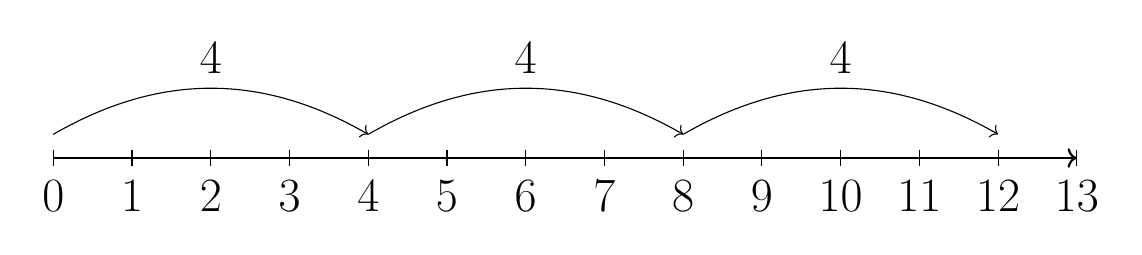
\begin{tikzpicture}
\draw[thick, ->] (0,0) -- (13,0) node[below] {$\ $};
\foreach \n in {0,1,2,3,4,5,6,7,8,9,10,11,12,13} {\draw (\n,0.1) -- (\n,-0.1) node[below] {$\n$};}
\draw[->, bend left=30] (0,0.3) to node[above] {$4$} (4,0.3);
\draw[->, bend left=30] (4,0.3) to node[above] {$4$} (8,0.3);
\draw[->, bend left=30] (8,0.3) to node[above] {$4$} (12,0.3);
\end{tikzpicture}
\end{center}

Practice counting by fives all the way to 100:\\
5, 10, 15, 20, 25, 30, 35, 40, 45, 50, 55, 60, 65, 70, 75, 80, 85, 90, 95, 100.\\

Practice counting by sixes all the way to 100:\\
6, 12, 18, 24, 30, 36, 42, 48, 54, 60, 66, 72, 78, 84, 90, 96.\\

Practice counting by sevens all the way to 100:\\
7, 14, 21, 28, 35, 42, 49, 56, 63, 70, 77, 84, 91, 98.\\

Practice counting by eights all the way to 100:\\
8, 16, 24, 32, 40, 48, 56, 64, 72, 80, 88, 96.\\

Practice counting by nines all the way to 100:\\
9, 18, 27, 36, 45, 54, 63, 72, 81, 90, 99.\\

Practice counting by tens all the way to 100:\\
10, 20, 30, 40, 50, 60, 70, 80, 90, 100.\\

\newpage

\section{Times tables}
Now learn the times table from 1 to 10.

\begin{center}
\begin{tabular}{|c||*{10}{c|}}
\hline
$\times$ & 1 & 2 & 3 & 4 & 5 & 6 & 7 & 8 & 9 & 10 \\
\hline\hline
1 & 1 & 2 & 3 & 4 & 5 & 6 & 7 & 8 & 9 & 10 \\
2 & 2 & 4 & 6 & 8 & 10 & 12 & 14 & 16 & 18 & 20 \\
3 & 3 & 6 & 9 & 12 & 15 & 18 & 21 & 24 & 27 & 30 \\
4 & 4 & 8 & 12 & 16 & 20 & 24 & 28 & 32 & 36 & 40 \\
5 & 5 & 10 & 15 & 20 & 25 & 30 & 35 & 40 & 45 & 50 \\
6 & 6 & 12 & 18 & 24 & 30 & 36 & 42 & 48 & 54 & 60 \\
7 & 7 & 14 & 21 & 28 & 35 & 42 & 49 & 56 & 63 & 70 \\
8 & 8 & 16 & 24 & 32 & 40 & 48 & 56 & 64 & 72 & 80 \\
9 & 9 & 18 & 27 & 36 & 45 & 54 & 63 & 72 & 81 & 90 \\
10 & 10 & 20 & 30 & 40 & 50 & 60 & 70 & 80 & 90 & 100 \\
\hline
\end{tabular}
\end{center}

\vspace{32pt}
Do it by saying the times table out loud, one column at a time, many times, until they can all be done without looking. Again, this works well when done as a group.\\

For each column, say "1 times 4 is 4. 2 times 4 is 8. 3 times 4 is 12. 4 times 4 is 16... and so on.\\

Then ask for the answer to random pairs of numbers, and do it until there is always an instant answer.\\

\newpage

\section{Multiplication in Columns}

To multiply larger numbers, arrange them into columns aligned on the units. Then you can multiply the columns separately into a product for the units, a product for the tens, a product for the hundreds, and so on. Then you add these products to get a final product.\\

\subsection*{Multiplying by a single number}

\begin{center}
\begin{tabular}{c@{\,}c@{\,}c@{\,}c@{\,}cl}
       &1,&2&3&4&\\
\times &  & & &6&\\
\cline{1-5}
       & &  &2&4&\ 1's product\\
       & &^{1}1&8& &\ 10's product\\
       &1&2& & &\ 100's product\\
     + &6& & & &\ 1000's product\\
\cline{1-5}
      &7,&4&0&4&\
\cline{1-5}
\cline{1-5}
\end{tabular}\\
\end{center}

See how there is a product for the units, a product for the tens, a product for the hundreds and a product for the thousands, and that they are lined up under those places.

\newpage
To make sure your products are in the right columns, and to make them easier to add up, fill in the blank spaces with zeroes.

\begin{center}
\begin{tabular}{c@{\,}c@{\,}c@{\,}c@{\,}c}
       &1,&2&3&4\\
\times  & & & &6\\
\hline
        & & &2&4\\
    & &^{1}1&8&0\\
        &1&2&0&0\\
      + &6&0&0&0\\
\hline
       &7,&4&0&4\\
\hline
\hline
\end{tabular}\\
\end{center}

\vspace{16pt}
And finally, you make this much shorter by doing the carries for the addition at the same time as you are working out the products.

\begin{center}
\begin{tabular}{c@{\,}c@{\,}c@{\,}c@{\,}c}
          &1,&2&3&4\\
\times &_1_&_2&_2&6\\
\hline
          &7,&4&0&4\\
\hline
\hline
\end{tabular}\\
\end{center}

\newpage

\subsection*{Multiplying any two numbers}
Multiply each digit of the number being multiplied by each digit of the number it is being multiplied by, starting at the right with the units.

\begin{center}
\begin{tabular}{c@{\,}c@{\,}c@{\,}c@{\,}cc}
       & & &2&3&\\
\times & & &3&4&\\
\cline{1-5}
       & & &1&2&\ $(4 \times 3)$\\
      +& & &8& &\ $(4 \times 2)$\\
\cline{1-5}
       & & &9& &\ $(3 \times 3)$\\
  +& &^{1}6& & &\ $(3 \times 2)$\\
\cline{1-5}
       & &7&8&2&\\
\cline{1-5}
\cline{1-5}
\end{tabular}\\
\end{center}

\vspace{32pt}
Again, fill in the blank spaces with zeroes to make sure numbers are kept in the correct columns and to make it easier to add up without errors.\\

\begin{center}
\begin{tabular}{c@{\,}c@{\,}c@{\,}c@{\,}c}
       & & &2&3\\
\times & & &3&4\\
\hline
       & & &1&2\\
       & & &8&0\\
       & & &9&0\\
  +& &^{1}6&0&0\\
\hline
       & &7&8&2\\
\hline
\hline
\end{tabular}\\
\end{center}

\newpage

And finally, this can be shortened by doing some of the carrying and adding while you're writing the partial products.

\begin{center}
\begin{tabular}{c@{\,}c@{\,}c@{\,}c@{\,}c}
       &&&2&3\\
\times &&&_{1}3&4\\
\hline
       &&&9&2\\
+ &&^{1}6&9&0\\
\hline
      &&7&8&2\\
\hline
\hline
\end{tabular}\\
\end{center}

\vspace{32pt}
And that is how you multiply.\\

\newpage

Here is longer example:

\begin{center}
\begin{tabular}{c@{\,}c@{\,}c@{\,}c@{\,}c@{\,}c@{\,}c}
       & & & &8&9&7\\
\times & & & &7&8&9\\
\hline
       & & & & &6&3\\
   & & & &^{1}8&1& \\
  +& & &^{2}7&2& & \\
\hline
       & & & &5&6& \\
       & & &7&2& & \\
  +& &^{2}6&4& & & \\
\hline
       & & &4&9& & \\
       & &6&3& & & \\
  +&^{2}5&6& & & & \\
\hline
      &7&0&7,&7&3&3 \\
\hline
\hline
\end{tabular}\\
\end{center}

\vspace{32pt}
See how there are partial products for the units, the tens, and the hundreds of the multiplier, each aligned with its digit of the multiplier.\\

\newpage

Padding with zeroes makes adding easier and prevents errors by keeping columns in line.

\begin{center}
\begin{tabular}{c@{\,}c@{\,}c@{\,}c@{\,}c@{\,}c@{\,}c}
       & & & &8&9&7\\
\times & & & &7&8&9\\
\hline
       & & & & &6&3\\
   & & & &^{1}8&1&0\\
  +& & &^{2}7&2&0&0\\
\hline
       & & & &5&6&0\\
       & & &7&2&0&0\\
  +& &^{2}6&4&0&0&0\\
\hline
       & & &4&9&0&0\\
       & &6&3&0&0&0\\
  +&^{2}5&6&0&0&0&0\\
\hline
      &7&0&7,&7&3&3\\
\hline
\hline
\end{tabular}\\
\end{center}

\vspace{32pt}
You can make this shorter by doing carries while working out the products. This is the usual way to do multiplication of large numbers by hand.

\begin{center}
\begin{tabular}{c@{\,}c@{\,}c@{\,}c@{\,}c@{\,}c@{\,}c}
           &&&&8&9&7\\
    \times &&&&7&8&9\\
  _6&_4&_7&_5&_8&_6&\\
\hline
  &&&^{1}8&^{1}0&7&3\\
     &&^{1}7&1&7&6&0\\
    &^{1}6&2&7&9&0&0\\
\hline
       &7&0&7,&7&3&3\\
\hline
\hline
\end{tabular}\\
\end{center}

\newpage

\subsection*{Multiplication with Decimal Points}
The number of digits after the decimal point of the product is the total of the number of digits after the decimal points of the numbers being multiplied.

Fill with trailing zeroes so that both numbers have the same number of digits after the decimal point.\\

\begin{center}
\begin{tabular}{c@{\,}c@{\,}c@{\,}c@{\,}c@{\,}c@{\,}c@{\,}c@{\,}c@{\,}c@{\,}}
       & & & & & &2&.&3&4\\
\times & & & & & &5&.&2&0\\
\hline
       & & & & & & & & &0\\
       & & & & & & & &0& \\
+      & & & & & &0& & & \\
\hline
       & & & & & & & &8& \\
       & & & & & &6& & & \\
+      & & & &4& & & & & \\
\hline
       & & & &2& &0& & & \\
   & &^{1}1& &5& & & & & \\
+      &1&0& & & & & & & \\
\hline
       &1&2&.&1& &6& &8&0\\
\hline
\hline
\end{tabular}\\
\end{center}

\newpage

Padding the partial products with zeroes makes the columns easier to see and can prevent errors, and you don't actually  need to multiply out the first zero.

\begin{center}
\begin{tabular}{c@{\,}c@{\,}c@{\,}c@{\,}c@{\,}c@{\,}c@{\,}c@{\,}c@{\,}c@{\,}}
       & & & & & &2&.&3&4\\
\times & & & & & &5&.&2&0\\
\hline
       & & & & & & & &8&0\\
       & & & & & &6& &0&0\\
+      & & & &4& &0& &0&0\\
\hline
       & & & &2& &0& &0&0\\
   & &^{1}1& &5& &0& &0&0\\
+      &1&0& &0& &0& &0&0\\
\hline
       &1&2&.&1& &6& &8&0\\
\hline
\hline
\end{tabular}\\
\end{center}

\vspace{32pt}
You can make this even shorter if you do carries while working out the products, and you don't really need to add the trailing zero to the multiplier as long as the decimal points line up.

\begin{center}
\begin{tabular}{c@{\,}c@{\,}c@{\,}c@{\,}c@{\,}c@{\,}c@{\,}c@{\,}c@{\,}c@{\,}}
       & & & & & &2&.&3&4\\
\times & &_1& &_2& &5&.&2& \\
\hline
       & & & &4& &6& &8& \\
  +&1&^{1}1& &7& &0& &0& \\
\hline
       &1&2&.&1& &6& &8& \\
\hline
\hline
\end{tabular}\\
\end{center}

\newpage
\
\newpage

\doublespacing

\begin{center}

Enquiries

\textbf{Applied Scholastics Ferndale}

Principal: Paula McLennan

mobile phone: 0431 683 306

email address: apsferndale@gmail.com

website: apsferndale.webs.com

\end{center}

\end{spacing}

\end{document}